\begin{definetable}{tab:rep}
    \begin{threeparttable}
    \centering
    \scriptsize
    \begin{subtable}{\columnwidth}
            \centering
            \scriptsize
            \begin{tabular}{r | c | c | c | c }
                \parbox{1cm}{\raggedleft Irradiance\\Trace} & Total Days & \parbox{1cm}{\centering Average\\Power\\(\textmu W/cm\textsuperscript{2})} & \parbox{1.6cm}{\centering 90\textsuperscript{th} Percentile\\Daily Power (\textmu W/cm\textsuperscript{2})} & \parbox{1.6cm}{\centering 10\textsuperscript{th} Percentile\\Daily Power (\textmu W/cm\textsuperscript{2})} \\\hline
                EnHANTS A   & 394  & 15.1     & 25.0      & 5.2\\
                EnHANTS D   & 311  & 97.4     & 256.5     & 24.8\\
                %Enhants C   & 327  & 745.4    & 1610.0    & 176.1\\
            \end{tabular}
            \caption{Indoor photovoltaic irradiance traces}
        \end{subtable}\\
        \vspace{-6pt}
        \begin{subtable}{\columnwidth}
            \centering
            \scriptsize
            \begin{tabular}{r | c | c | c}
                Workload Class & Energy per Event (uJ) & Average Period & Average Power (\textmu W)\,\tnote{a}\\\hline
            \multirow{4}{*}{Periodic}   & \multirow{4}{*}{586}  & 10\,s                 &  58.6     \\
                                        &                       & 30\,s                 &  24.5     \\
                                        &                       & 60\,s                 &  14.7     \\
                                        &                       & 120\,s                &  9.8      \\\hline
            \multirow{3}{*}{Reactive}   & \multirow{3}{*}{86}   & 3.4\,s\,\tnote{b}     &  25.3     \\
                                        &                       & 6.8\,s\,\tnote{b}     &  17.6     \\
                                        &                       & 13.6\,s\,\tnote{b}    &  11.3     \\\hline
                 Long-Running           & 93,300                 & 2\,weeks\,\tnote{c}  &  5.1      \\
            \end{tabular}
            \caption{Representative workloads}
        \end{subtable}
    \end{threeparttable}
    \vspace{-4pt}
    \begin{tablenotes}[para]
    \scriptsize
    \item[a] Average power includes an average 5\,\textmu W idle power, measured in \cref{sec:impl:permamote}.\\
    \item[b] Event times are based on a Poisson distribution for each hour of the day and drawn every second. The distribution is parameterized by collected entryway data then scaled.\\
    \item[c] Event time is based on a uniform distribution and drawn every second.
    \end{tablenotes}
    \caption{\normalfont Representative harvesting conditions and workloads.
    To evaluate different energy storage architectures, we define a set of energy harvesting
    conditions and workloads that are representative of common sensing applications. We choose two
    real, 1\,Hz, irradiance traces with different magnitudes of available energy. We define three
    workloads: periodic, reactive, and long-running, and we characterize those workloads
    for different event frequencies. The energy used for each event is measured
    on our reference hardware described in \cref{sec:impl:permamote}.
    }
\end{definetable}

\begin{definefigure}{fig:framework}
  \centering
  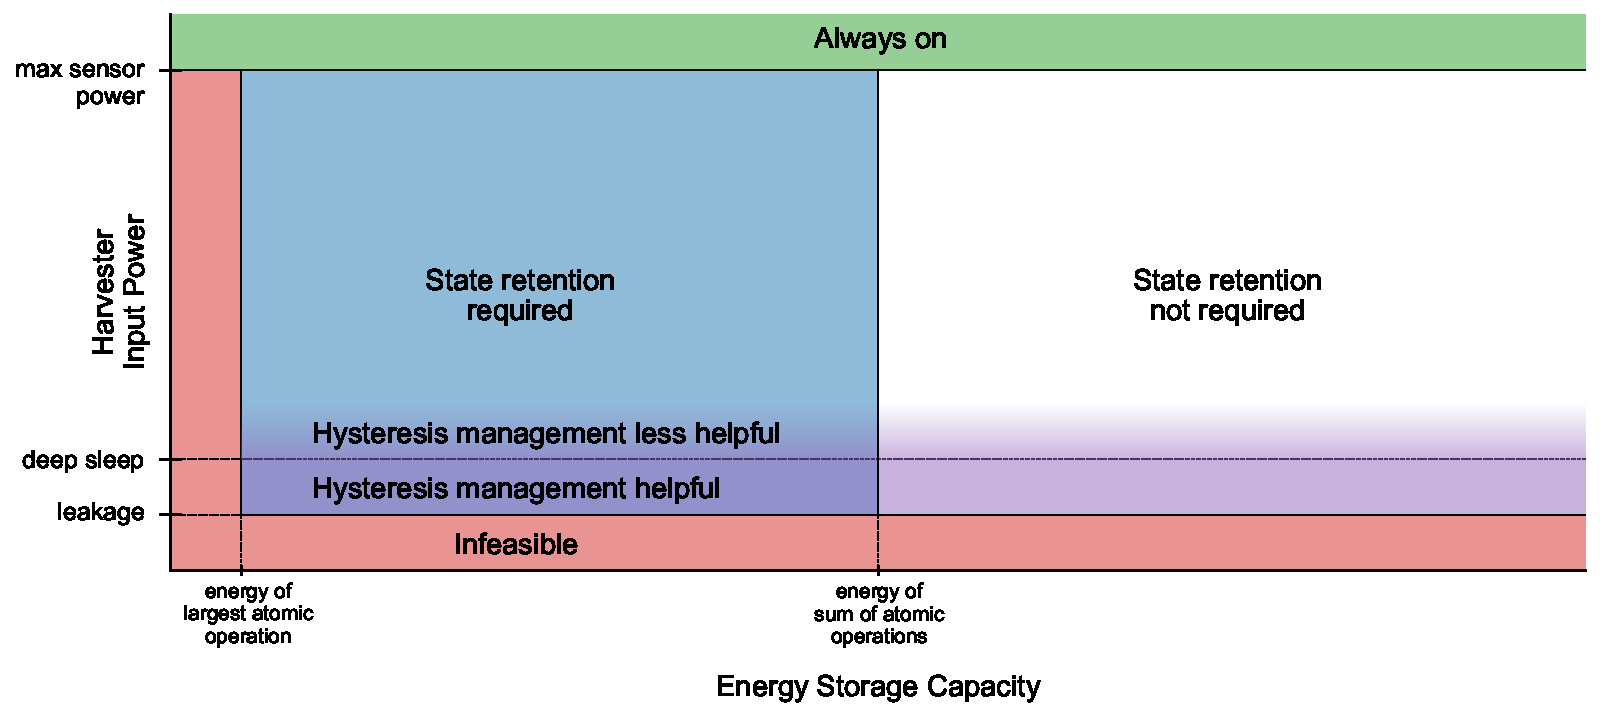
\includegraphics[width=\columnwidth]{figs/capacity/harvesting_framework/framework}
  \caption{
  %Energy harvesting
  %sensors have different capabilities and requirements
  \normalfont Design space for energy harvesting sensors based on their energy
  income (which we assume is constant for this analysis), energy storage capacity, and workload.
  Workload is represented by the largest atomic/non-atomic operations supported
  by a design, as well as the deep sleep and leakage power.  The plot breaks
  into four regions: \textbf{1)} always
  on or effectively powered, \textbf{2)} Infeasible due to lack of energy storage or
  leakage higher than harvesting rate \textbf{3)} Feasible but requires checkpointing
  to make forward progress, and \textbf{4)} Enough energy storage to not require
  or benefit from checkpointing. Additionally, sensors which have high
  power when they enter deep sleep before depleting their
  energy buffer may benefit from hysteresis management techniques.
  This benefit diminishes with lower sleep currents and higher harvesting potential.
  %With increased capacity, sensors can avoid the complexity of intermittent
  %programming techniques and specialized, reconfigurable power supplies in addition
  %to the other benefits of increased capacity discussed
  %in \cref{sec:store}.
  }
\end{definefigure}

\begin{definetable}{tab:parameters}
    \centering
    \begin{adjustbox}{width=\columnwidth}
    \begin{tabular}{lll}
\hline
\textbf{Config Type}& \multicolumn{1}{l}{\textbf{Parameter}}                   & \multicolumn{1}{l}{\textbf{Description}} \\ \hline
\textbf{Device}     & \texttt{operating\_voltage}                              & Output voltage of the power subsystem    \\
                    & \texttt{boost\_efficiency}                               & Efficiency of the boost converter        \\
                    & \texttt{frontend\_efficiency}                            & Efficiency of the harvesting frontend    \\ \hline
\textbf{Secondary}  & \texttt{capacity}                                        & Capacity of secondary in joules or mAh   \\
                    & \texttt{esr}                                             & Equivalent series resistance in ohms     \\
                    & \texttt{leakage\_constant}                               & Factor for capacity dependent leakage    \\
                    & \texttt{\string{max, min\string}\_hyst}                  & Secondary capacity upper/lower hysteresis\\ \hline
\textbf{Primary}    & \texttt{capacity}                                        & Capacity of primary in mAh               \\
                    & \texttt{leakage\_percent}                                & Percent capacity leakage per year        \\ \hline
        \textbf{Harvester}  & \texttt{area}                                    & Area of solar harvester in cm\textsuperscript{2}\\
\textbf{(Solar)}    & \texttt{efficiency}                                      & Efficiency of solar panel                \\ \hline
%\textbf{Workload}   & \texttt{type}                                            & Periodic or Reactive                     \\
%                    & \texttt{period/scale}                                    & Period, or scale for average \# of events \\
%                    & \texttt{opportunistic}                                   & Ignore period, and perform events ASAP   \\
%                    & \texttt{sleep\_current}                                  & Current draw of system in low power mode \\
%                    & \texttt{startup\_\string{energy, period\string}}         & Energy, time required for startup        \\
%                    & \texttt{event\_\string{energy, period\string}}           & Total energy, time required for work event \\
%                    & \texttt{atomic}                                          & Workload is atomic, or intermittent      \\
%                    & \texttt{event\_period\_min}                              & If not atomic, minimum splitable period  \\ \hline

    \end{tabular}
    \end{adjustbox}
    \caption{\normalfont Simulation configuration parameters.
      A representative set of available configuration options for our
      simulation of a sensor with secondary storage and energy harvester, a
      primary-cell, or both. A secondary-cell can be configured with a
      hysteresis, with a lower bound set to \texttt{min\_hyst}
      and an upper bound of \texttt{max\_hyst}.
      %This upper bound must represent
      %the minimum amount of
      %energy to do useful work.
      %Therefore, the upper bound of charging
      %hysteresis is set to \texttt{secondary\_max\_hyst}.
      %Workloads are
      %configured to be either periodic or reactive, and workload intensity is
      %determined by period, or a scaling factor determining the average number
      %of events picked from a random distribution.
      }
\end{definetable}
\begin{definefigure}{fig:statemachine}
    \centering
    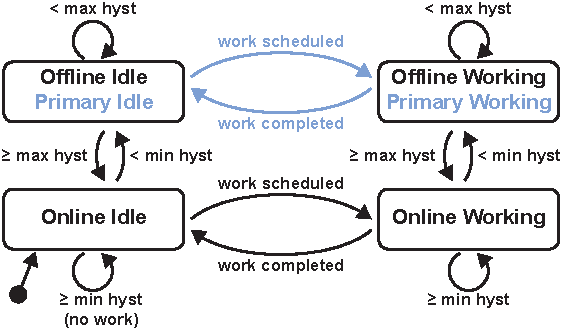
\includegraphics[width=\columnwidth]{figs/capacity/model_state_machine}
    \caption{\normalfont Model state machine.
    A modeled device can be in one of four states: \textsf{Offline Idle},
    \textsf{Online Idle}, \textsf{Online Working}, and \textsf{Offline
    Working}. When a device is \textsf{Offline Idle}, it has run out of energy
    and is off. If a device is \textsf{Online
    Idle}, it is on and in deep sleep, ready to perform work if triggered. If
    triggered, a device moves to \textsf{Online Working}, where it performs a
    portion of a work event.  If a workload is atomic, workload events
    \textit{must} be completed in one \textsf{Online Working} step, without any
    transitions to an offline state.  \textsf{Offline Working} means that while
    working on a non-atomic task, the device ran out of energy, checkpointed,
    and is waiting to harvest more and resume its task.  For devices
    configured with a primary-cell, \textsf{Offline Idle} and \textsf{Offline
    Working} become \textsf{\textcolor{primary-blue}{Primary Idle}} and
    \textsf{\textcolor{primary-blue}{Primary Working}} respectively.  In these
    states, outgoing energy is charged against the primary-cell and the device
    remains online and able to perform work for the life of the primary-cell.
    %State transitions are determined by incoming energy, the state of charge of
    %the secondary storage, and the generated work schedule from workload
    %parameters.
    }
\end{definefigure}

%1) If the energy harvester supplies the sensor
%  with more power than its peak power requirement, then it is always on, otherwise it
%  must have some capability of storing energy for later use in an energy buffer.
%  2) If this storage capacity is less than the amount required to perform an
%  atomic operation (such as boot or send a radio packet),
%  then the energy will run out before the operation is completed
%  and the operation is Infeasible. If the energy harvester is supplying less
%  power than the leakage power of the sensor it will never accumulate stored energy.
%  3) If the energy buffer can hold enough energy to perform atomic operations, but
%  not enough to complete a more complex tasks composed of multiple, dependent
%  atomic operations (such as sample a sensor then send a radio packet), then
%  some mechanism of saving state and continuing progress on the next reboot
%  must be employed.
%  4) If the amount of power consumed when a sensor willfully powers down
%  (referred to as deep sleep) is a substantial portion of the harvested energy,
%  then it is often beneficial to continue operating until the energy
%  buffer is depleted rather than stop early to slowly recharge.
%  Under this scenario hysterysis management techniques
%  such as reconfigurable capacity and task-capacity coupling can increase sensor
%  performance. The amount of help these techniques provide lessens with
%  lower deep sleep power and higher harvesting potential.
%  5) If none of these conditions are true then a sensor can operate without
%  intermittent techniques, moving in and out of sleep mode to accomplish its
%  tasks. Greater capacity has additional benefits even when in this regime.



\\


%and does not highlight the
%benefits of capacity. Increased energy capacity allows more energy utilization
%in periods of superfluous energy which then can be used in periods of energy
%drought or for high-intensity or long running operations. Additionally, this
%framework does not show the benefits afforded by a backup energy store, which
%can provide increased reliability similar cases. With increased energy
%capacity, designs should also expect increased self-discharge currents, and
%this is not reflected in the framework. Also, a large energy storage will
%increase cold start time from completely empty storage, but if energy is
%managed well, this state is rare.

%\hl{Discussion about non-rechargeable effects?}

%To account for energy variability and examine capacity's effect on reliability,
%in the next section we explore these facets with a data-driven numerical model.

\section{Modeling the Common Case}
\label{sec:overview}
%To compare the relative performance of different energy storage
%architectures and reevaluate assumptions about the use of batteries in energy
%harvesting sensors,
The framework we have presented does not consider
harvesting and workload
variability.
To explore the dynamic effects that energy
capacity and backup storage have on sensor performance in the face
of variability, we develop a simple numerical model.
%we define both the
%conditions and the key metrics which form the basis of the
%analysis.
%Our goal is to analyze these energy storage architectures for the most
%common application scenarios and environments, so this section defines what we consider
%the common case for energy harvesting sensors.
%Additionally, we describe the
%simple numerical model we use to explore energy utilization and its effect on
%reliability and capability in these workloads.\\
We use representative environmental conditions, measurements of real hardware,
and synthesized workloads to determine the common case for our model and simulate
the behavior of energy harvesting sensors. From these data, our model
produces estimates of energy utilization, availability, responsiveness, and
lifetime.
%Since many modern sensor nodes exhibit lifetimes of months, years, or
%are theoretically infinite, it is infeasible to perform this analysis
%strictly through experimentation, so we must also define the methods
%by which we model their behavior in order to expose long-term trends.\\
\\

\vspace{-6pt}
\noindent
\textbf{Environmental Conditions.}
%\hl{we need to figure out where to argue the reasons energy harvesting is viable and worth it now, vs a few years ago - not sure here is the best place}
%Energy harvesting is a viable life-extending addition to a sensor node.
%New components enable systems with lower average power that is closer to, at,
%or under that of ambient indoor light. (provide examples of soc, sensors, etc on permamote, and average power of low light indoor enhants trace)
%\hl{why indoors? need to motive that this is the common case}
%This sensor is designed to perform
%dynamic, high-fidelity indoor lighting control, so we constrain our analysis to
%this environment.
We
assume an indoor environment
that is built for and used
by people.
Occupied indoor environments are the focus of a significant
amount of
prior work, %in applied sensor networks
and for good reason: most
applications aim to improve the lives of people and are necessarily present
in the spaces they occupy. Even the example applications of intermittent,
energy harvesting systems are nearly all centered around monitoring
indoor and human-centric phenomena~\cite{hesterTimely17,hesterFlicker17,colinReconfigurable18,campbellEnergy14}.
We expect our environment to be lit, and that it may
occasionally get direct or indirect sunlight. We use
indoor photovoltaic energy harvesting because under these conditions,
it offers an order of magnitude more energy than other methods.
This does not mean that the conclusions we draw are not applicable to other
environments and harvesting methods, but that the sizing and lifetime
conclusions may be different.

To model the harvestable light in an occupied indoor environment, we use
the EnHANTS indoor irradiance dataset~\cite{gorlatova2013networking}. We
find that it is the most complete and extensive dataset for indoor light
irradiance traces, capturing over a year of data in several situations.
The traces we use for our model are summarized in \cref{tab:rep}.\\

\vspace{-6pt}
\noindent
\textbf{Representative Hardware.}
We limit our analysis to the effects of capacity,
independent of the differences of energy intensity or efficiency in device
component selection. To do so, we define an example solar energy harvesting
sensor platform that utilizes available, state-of-the-art, commercial
components.
\placefigure[t]{tab:rep}
%We implement this platform as described in
%\cref{sec:impl:permamote} and
%use it to inform the energy requirements and harvesting capabilities
%of the following workloads and energy harvesting traces.
We choose new
components in an attempt to better represent prior energy storage designs and
give them the benefit of the improvements that have occurred in recent years.
We take benchmark
measurements of various tasks performed by this platform, such as the
amount of time and energy required to sample a sensor or send a Bluetooth Low
Energy (BLE) packet. These benchmarks are used to generate energy utilization metrics
for our representative workloads shown in \cref{tab:rep}.
The physical size of the solar panel used by this sensor
is assumed to be
10.9~cm\textsuperscript{2} and the volume of the sensor node is similar to prior
work like the Hamilton sensor~\cite{kim2018system}.
We implement this design and describe it further in \cref{sec:impl:permamote}.
\\

\vspace{-6pt}
\noindent
\textbf{Representative Workloads.}
We find that sensing workloads generally fall into three
categories: (i) periodic sense-and-send~\cite{mainwaring2002wireless}, (ii) reactive event detection~\cite{campbellEnergy14}, and (iii) infrequent,
long-running, high-power events~\cite{levis2004trickle}. We choose a representative workload for each
of these categories to use in our model.
%Periodic sense and send represents the node
%waking up, sampling a sensor, sending the collected data wirelessly, and
%returning to a sleep state. This workload is a classic application for wireless
%sensor networks \cite{mainwaring2002wireless, yick2008wireless}. Reactive event detection
%represents workloads in which the sensor reacts to some phenomena, like motion
%or an anomalous sensor reading. This workload is also well represented in past work \cite{campbellEnergy14, liang2009racnet}.
%Workloads like cryptographic key exchanges and over-the-air (OTA) firmware
%updates represent infrequent, relatively expensive operations (in both time and
%energy).
We characterize our ``periodic sense-and-send''
workload as periodically sampling a light and color sensor and sending a
BLE
advertisement containing the data.
Our ``reactive workload'' is
represented by sending a BLE advertisement upon motion detection of the main
entrance of a university building, and we linearly scale the frequency
of these events to represent varying amounts of usage. We treat these
workloads as atomic.  Finally, our ``infrequent expensive'' workload is a
contiguous
task that is representative of an
over-the-air firmware update, which is randomly executed with an average occurrence rate
of once every two weeks.
We conservatively assume these long running tasks can be interrupted
and resumed at any point during execution and that any checkpointing is free.
%A summary of these workloads is presented in \cref{tab:rep}.\\
\\

\vspace{-6pt}
\noindent
\textbf{A Predictive Model.}
We use the previously discussed indoor irradiance traces, generalized
workloads, and hardware characterizations to model the behavior of sensors
using different types and sizes of energy storage. We develop an open
source\footnote{\url{https://github.com/lab11/permamote/tree/master/simulator}}
numerical model that allows parameterization of various system
characteristics, including regulator efficiency, solar harvester size
and efficiency, energy storage capacity, leakage, ESR, and charge-discharge
efficiency. These parameters are summarized in \cref{tab:parameters}.

The simulation of our model operates as a second-by-second calculation of the
amount of energy entering and exiting a device.
At every step, the simulation calculates the net energy gain or loss of the
system based on its current state and available stored energy.  Occasionally,
the model performs a workload event based on either a periodic schedule (in the
case of a sense-and-send workload) or from a random distribution (reactive
event detection or a high-power event). For our modeling, workload schedules
are generated from values listed in \cref{tab:rep}.
%At every step, our
%simulation stores the state of charge for the secondary and primary storage,
%the amount of harvested energy that was used by the system, the total amount of
%available harvestable energy, the amount of successful and total events,
%and event time-to-completion. We perform linear regression on the resulting
%state of charge data for the primary storage, if it exists, to estimate
%lifetime of the system. Even though the system operates on second increments, we
This simulation is performed for the entirety of an
input irradiance trace, which constitutes about a year of data. During
a simulation, metrics such as energy utilization, the fraction of completed
events versus expected events, and events' time to completion are collected,
and if applicable, the primary-cell lifetime is estimated from a trace of its
state of charge.
%over the entire simulation.

During simulation, modeled devices can be online or offline and idle or performing
work. These states are shown in \cref{fig:statemachine}.  A device's state
transitions from top to bottom of this figure and vice versa depending on the
energy state of the secondary storage.
If the secondary-cell energy state drops below \texttt{min\_hyst},
%(the
%secondary state of charge goes below the configured
%\texttt{secondary\_min\_percent})
the state of the system moves to the upper
half (offline) of this diagram. The state of the system moves downward (online)
if the state of charge of the secondary reaches the \texttt{max\_hyst}
limit. Secondary charging hysteresis limits are defined by parameters described in \cref{tab:parameters}.
%The upper hysteresis limit is determined by the configured upper limit
%(\texttt{secondary\_max\_percent}) or if larger, the amount of energy required
%to start up (\texttt{startup\_energy}) and the configured minimum required
%amount of work (\texttt{event\_period\_min}).
A device's state can also move
to the right or left of the state machine depending on whether a workload event
is scheduled, or the prescribed workload has been completed. A new
workload event is counted as failed if the device is not in the \textsf{Online
Idle} state when it begins.
In the case of the ``atomic''
sense-and-send and reactive workloads, the modeled device will only begin
to perform an expected workload event if it has
enough energy to perform the event in entirety. If the workload is not atomic,
the device will only begin scheduled work if it has enough energy to make the
configured minimum amount of progress. We
make the assumption that the duration of atomic events are less than the one
second simulation step.
We assume that a modeled sensor has perfect, zero-energy progress
latching and can go to sleep at any point after an active event. If
there is energy remaining after performing a task, the modeled sensor will
attempt to spend the rest of the simulation period in the \textsf{Online Idle} state.

If the simulated device is configured with a backup primary-cell, offline
states transform to "primary" states in which the device remains on and
able to perform work, but charges energy usage to the primary storage instead
of the secondary. During these periods, the secondary cell continues charging
from harvested energy. Upon reaching the upper charging hysteresis
limit, the device returns to an online state, using energy stored in the
secondary.  If the primary storage is depleted, the simulation ends early.

%Incoming energy is calculated from irradiance measurements from the EnHANTs
%traces and both the efficiency of the solar panel (19\%) and harvesting front
%end (80\%). Outgoing energy depends on the whether the device is in an online
%or offline state, and constitutes the energy required for the device to start
%up, sleep, or perform active work.  Outgoing energy is modified by regulator
%and energy storage charge-discharge efficiency and includes estimated
%self-discharge based on the commonly used C/10,000 self-discharge constant for
%batteries~\cite{zimmermanSelf04}, and reported leakage for capacitors and
%supercapacitors from datasheets~\cite{tantalumDatasheet, ceramicDatasheet,
%murataCap, kemetCap}.

%Sometimes, the remaining amount of energy stored is not sufficient
%to remain in a sleep state on subsequent modeling periods and if the modeled
%sensor is not configured with back up primary storage, it will run out of stored
%energy and power off. The modeled sensor will then need to harvest enough
%energy to start up and continue operation.




%To evaluate this behavior, most important metric we wish to estimate
%is reliability. Of all the tasks we expected the device to perform, which did
%it complete successfully?
%For long-running, interruptible operations, how long
%did it take, and how long could it have taken if we had infinite energy available?
%Secondly, we also want to measure lifetime. For most energy
%harvesting devices this metric remains theoretically infinite or sufficiently
%long such that they are difficult to calculate based on existing evidence. For
%systems that employ primary-cells, it can be defined as the expected lifetime
%of the primary storage.

%For systems that use both, this metric becomes slightly unclear, as
%the device will likely continue to perform tasks in the absence of primary
%storage, but at a degraded performance.

%We should use the section to define our experiments. What workloads
%are we running, how are they representative, what datasets are we using
%for energy income, what size solar panel are we assuming. These choices
%should be well motivated by prior work such that it doesn't unfairly represent
%their intent
%
%We have already identified several types of workloads:
% - Periodic Sense and Send
% - Event detection and processing
% - Infrequent, high-power events/maintenance (maybe should be mixed with the other two?)
%
%Table: A table of the specifics about these workloads and the power we
%are assuming each part of the workload will consume. We should be liberal
%with power consumption so that systems we are comparing against are shown
%in the best possible light.

\placefigure[t]{tab:parameters}
\placefigure[t]{fig:statemachine}
\placefigure[t]{fig:usage}
